% This is samplepaper.tex, a sample chapter demonstrating the
% LLNCS macro package for Springer Computer Science proceedings;
% Version 2.20 of 2017/10/04
%
\documentclass[runningheads]{llncs}
%
\usepackage[utf8]{inputenc}
\usepackage{listings}
\usepackage{xcolor}
\usepackage{graphicx}
\usepackage{tabularx}
\usepackage{hyperref}
\usepackage{subcaption}

\graphicspath{ {./images/} }
\hypersetup{
    colorlinks=true,
    linkcolor=blue,
    filecolor=blue,
    citecolor=blue,
    urlcolor=blue,
    linktocpage=true
}
\setcounter{tocdepth}{2} %show more in the toc

\newcommand{\kw}[1]{\texttt{#1}}
\renewcommand{\contentsname}{table of content}
\usepackage{indentfirst}
\usepackage[english]{babel}

% If you use the hyperref package, please uncomment the following line
% to display URLs in blue roman font according to Springer's eBook style:
\renewcommand\UrlFont{\color{blue}\rmfamily}

%

\title{Infra-estrutura de Testes para Implementações de Referência do Standard ECMAScript}
\subtitle{}

%
\titlerunning{Live Metadata for Test262}
% If the paper title is too long for the running head, you can set
% an abbreviated paper title here
%
\author{Diogo Costa Reis\\ist187526\\
\email{diogo.costa.reis@tecnico.ulisboa.pt}}
%
\authorrunning{Diogo Costa Reis}
% First names are abbreviated in the running head.
% If there are more than two authors, 'et al.' is used.
%
\institute{Instituto Superior Técnico\\
Av. Rovisco Pais, 1\\
1049-001 Lisboa\\
Tel: +351 218 417 000\\
\email{mail@tecnico.ulisboa.pt}}
%


\begin{document}

% a solution to remove title and author from appearing in the table of contents: https://tex.stackexchange.com/a/318220
{\def\addcontentsline#1#2#3{}\maketitle}

%
\begin{abstract}
% TODO

\keywords{ECMAScript \and Specification Language \and Reference Interpreters \and Test262}
\end{abstract}


\newpage

\tableofcontents

\newpage

\section{Introduction}
\label{sec:Introduction}

\section{Goals}
\label{sec:Goals}

\section{Background}
\label{sec:Background}
This chapter provides an overview on the ECMAScript standard, the Test262 that are used to test the correct implementation of the ECMAScript standard, and finally an outline of the new metadata generated.

\subsection{ECMAScript}
\label{subsec:ECMAScript}
% overview da linguagem JS

% paragrafo - porque e' que javascript e' relevante (uma das linguagens mais usadas no momento)
JavaScript (JS) is a programming language mainly used in the development of client side web applications, also being one of the most popular programming languages. According to both GitHub and StakeOverflow statistics, JavaScript finished 2021 as second most active languages on GitHub\footnote{Second most utilized language based GitHub pull requests - https://madnight.github.io/githut/} as well as on StackOverflow.\footnote{Tendencies based on the Tags used - https://insights.stackoverflow.com/trends}



% Boa!
% Existem muitas implementacoes diferentes da linguagem: client-side (browsers), server-side (Node.js), embedded devices (Jerryscript) -> Estas implementacoes têm de estar de acordo no comportamento observavel -> é particularmente importante na Web -> senao temos sites que em ...
% -----------------------
% overview do standard -> descrita num standard
% Porque é muito importante que as várias implementacoes da linguagem coincidam -> o JavaScript está especificado num documento semi-formal que ...
% Falar sobre o standard
%   - o standard está como um interpretador de JavaScript em
%     pseudo-codigo - descreve detalhadamente os passos que
%    um interpretador de JS tem de executar ao avaliar qualquer
%    statement da linguagem
% Falar sobre o comité -  quem controla a evolucao do ECMAScript
ECMAScript standard\cite{ECMAScriptStandard} is the official document, written in the English language, in which the JavaScript language is defined. This document is in constant evolution, being updated by the ECMA Technical Committee 39 (TC39), which is responsible for maintaining the standard. The standard is currently in its twelfth version.
%
The standard specifies the \texttt{JavaScript} language, to ensure its multiple compilers and interpreters implementations are coherent. Some of the \texttt{JavaScript} compilers are the Hop~\cite{Hop} and the JSC~\cite{JSC} compilers, the most popular interpreters are Node.js~\cite{Node.js} and SpiderMonkey~\cite{SpiderMonkey}. These are only four implementations among many others, which come along with the many use cases that \texttt{JavaScript} has.
%
\texttt{JavaScript} is mostly used in the web context, both client-side within browsers and server-side, but also in embedded devices. Since \texttt{JavaScript} is used in so many scenarios and across so many different contexts, it is highly important that ECMAScript standard is defined in great detail to ensure consistency. Browsers, for example, need to run \texttt{JavaScript} implementations that coincide so that websites are correctly rendered and exhibit the same behavior. In order to achieve coherent implementations, the standard defines the types, values, objects, properties, syntax, and semantics of \texttt{JavaScript} that must be the same in every \texttt{JavaScript} compiler and interpreter, while allowing \texttt{JavaScript} implementations to define additional types, values, object, properties, and functions.




% Good, more detail if there is time
% Estrutura do standard
The \texttt{JavaScript} language can be divided into three major components, those being expressions and commands, built-in libraries, and finally internal functions.
%
\begin{itemize}
\item Expressions and commands describe the behavior of static constructions, detailing the semantics of the diverse expressions (e.g., assignment expressions, built-in operators, etc.), commands (e.g., loop commands, conditions command, etc.), and built-in types (Undefined, Null, Boolean, Number, String and Object).
%
\item The internal functions of the language are used to define the semantics for both expressions and commands, as well as the built-in libraries. Internal functions are not exposed beyond the internal context of the language. In other words, no JavaScript program uses internal functions directly.
%
\item Finally, built-in libraries encompass all the internal objects available when a JavaScript program is executed. Internal objects expose many functions implemented by the language itself, including functions to manipulate numbers, text, arrays, objects, among other things.
\end{itemize}


% MetaParagrafo tres tipos
\colorbox{orange}{The remaining} subsection provides a description of the three types of artifact described in the standard.
% QUESTION ainda nao foi lido pelo prof

% Expressions and statements
% Exemplo do standard  e explicacao (if)
\paragraph{Semantics of IF statement}
Figure \ref{fig:If-Else Statement} shows a snippet of the ECMAScript standard description of the \texttt{IF} command. In order to evaluate \texttt{IF} commands with the shape:

\begin{center}
\texttt{if (Expression) Statement1 else Statement2}
\end{center}

\noindent the language begins by evaluating the \texttt{Expression} storing the result in the variable \texttt{exprRef} (step 1). The previous step will be used as Boolean, therefore, the result of the previous step will be converted to a Boolean using the internal functions \texttt{ToBoolean} and \texttt{GetValue}, and having the result stored in the variable \texttt{exprValue} (step 2).A different \texttt{Statement} will be followed depending on \texttt{exprValue}. If \texttt{exprValue} has the value \texttt{true} the variable \texttt{stmtCompletion} will have the evaluation of the first \texttt{Statement} (step 3). Otherwise, the variable \texttt{stmtCompletion} will store the result of evaluating the second \texttt{Statement} (step 4). Finally, a \texttt{Completion} will be returned, if the \texttt{stmtCompletion} has non empty value then it will be returned, however, when the value is empty it will be replaced with undefined (step 5).

\begin{figure}[ht]
    \centering
    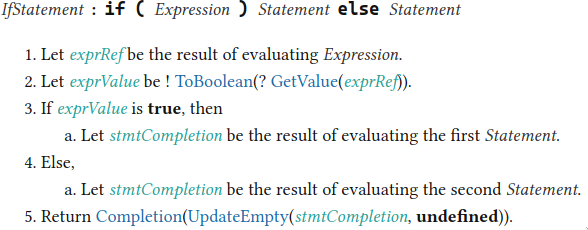
\includegraphics[width=0.8\textwidth]{images/if_statement.png}
    \caption{ECMAScript definition of an if-else statement}
    \label{fig:If-Else Statement}
\end{figure}

% arrays são objetos como os outros
% arrys tem propriedades especiais
% example of Array.pop
% Built-ins (Array.pop)
% printscreen do standard e explicacao
\paragraph{Semantics of the Pop function}
The Array built-in is an object as any other in JavaScript. The main difference is in its properties. Array Objects have a property \texttt{length} that contains the size of the array, as well as a property for each element of the array (from zero to \texttt{length} minus 1).

Figure \ref{fig:Array_pop_example} shows a simplified version of an array performing the pop function, where \texttt{(a)} and \texttt{(b)} are the before and after respectively.
Before preforming \texttt{pop} \texttt{(a)}, the array has three  properties \texttt{length}, \texttt{0}, and \texttt{1}. Property \texttt{length} represents the size of the array that has value \texttt{2}, while the properties \texttt{0} and \texttt{1} store the first (\texttt{banana}) and second (\texttt{kiwi}) elements of the array respectively.
After \texttt{pop} is preformed \texttt{(b)}, the last element is of the array is removed (highlighted in red at \texttt{(a)}) and the \texttt{length} property (highlighted in green) is decremented by one since the size of the array changes to one.

% TODO change length with quotation marks
\begin{figure}[ht]
    \centering
    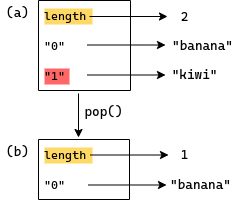
\includegraphics[width=0.4\textwidth]{images/array_pop_example.png}
    \caption{Example Array.pop}
    \label{fig:Array_pop_example}
\end{figure}
Figure \ref{fig:Array_pop} shows a snippet of the ECMAScript standard description of the pop function in the Array Built-in. To begin with, the array will be converted to and Object using the \texttt{ToObject} function, and stored in the \texttt{O} variable (step 1).
Afterwards, the array length of the previously calculated variable will be calculated with the \texttt{LengthOfArrayLike} internal function, and storing the result in the \texttt{len} variable (step 2).
At this point there are to ways to proceed depending on the value of \texttt{len}. If the value is zero, the Array is empty, then the property \texttt{length} of \texttt{O} is set to zero and \texttt{undefined} is returned (step 3).
Otherwise, when \texttt{len} is different from zero, meaning that the Array is not empty, the Array's last element will be removed (described in Figure \ref{fig:Array_pop_example}) and returned (step 4).
To begin with, the language will assert that \texttt{len} is positive (step 4.a).
Afterwards, the \texttt{newLen} variable will store the value of \texttt{len} decremented by 1 (step 4.b).
The variable \texttt{index} will store the variable calculated in the previous step represented as a String converted with the \texttt{toString} function (step 4.c).
Then, stores the value of the \texttt{O} variable at the property corresponding to \texttt{index} in the \texttt{element} variable using the \texttt{Get} function (step 4.d).
Subsequently, deletes the previously mentioned property of the \texttt{O} variable with the \texttt{DeletePropertyOrThrow} function (step 4.e).
In addition, sets the \texttt{length} property of the \texttt{O} variable  to the \texttt{newLen} using the \texttt{Set} function (step 4.f).
Finally, returning the value of the variable \texttt{element} (step 4.g).

\begin{figure}[ht]
    \centering
    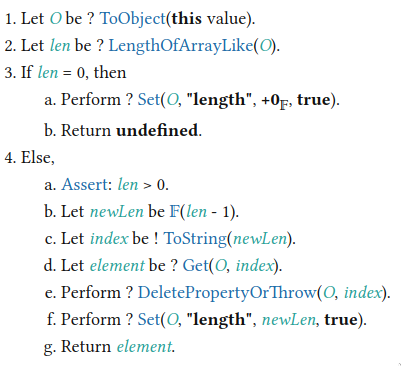
\includegraphics[width=0.6\textwidth]{images/array_pop.png}
    \caption{ECMAScript definition of Array.pop}
    \label{fig:Array_pop}
\end{figure}



% Internal Functions (LenghtOfArrayLike)
% printscreen do standard e explicacao
\paragraph*{LengthOfArrayLike internal function}
Figure \ref{fig:LengthOfArrayLike} shows a snippet of the ECMAScript standard description of the \texttt{LengthOfArrayLike} internal function, that evaluates the function:

\begin{center}
\texttt{LengthOfArrayLike (obj)}
\end{center}

\noindent The language starts by asserting that \texttt{obj} is an \texttt{Object} (step 1). Afterwards, gets the value of the property \texttt{length} from \texttt{obj} using the function \texttt{Get}. Then, converts the previously mentioned value to an Integer that represents the length with the \texttt{ToLength} function, and finally returns said Integer (step 2).

\begin{figure}[ht]
    \centering
    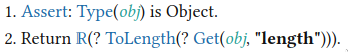
\includegraphics[width=0.5\textwidth]{images/length_array_like.png}
    \caption{ECMAScript definition of the LengthOfArrayLike}
    \label{fig:LengthOfArrayLike}
\end{figure}




\subsection{Test262}
\label{subsec:Test262}


% paragrafo - JS tem muitas particularidades que dificultam o desemvolvimento e testagem  -> É muito dificil desenvolver
% novas implemenentacoes da linguagem
% Existe uma bateria de testes que testa as implementacoes da
% linguagem contra o standard
% Esta bateria de testes é dificil de manter
% Porque? - muitos testes, muitas features, em geral ha retrocompatibilidade mas ha um pequeno numero de casos onde a retrocompatibilidade nao se verifica -> os testes de ser modificados
Implementing a \texttt{JavaScript} engine is particularly difficult since it involves dealing with the many corner cases that exist in the language. To test that corner cases are correctly dealt with there is \texttt{Test262}\cite{Test262}, the ECMAScript standard test battery. Although, \texttt{Test262} is vital to the \texttt{JavaScript} engines, it is very hard to maintain due it's complexity, the total number of tests is around \colorbox{orange}{39837} divided into \colorbox{orange}{87} subfolders, each correspond to roughly one section of the standard. \texttt{Test262} complexity grows with changes to the standard since in most cases backward compatible is maintained except for a few select cases. 
% 87 subfolders on built-ins + language
% QUESTION round number? (40000)
% QUESTION 105 subfolders if add intl402 (which also has files that were ignore)



% Implementacoes parciais da linguagem 
% Na acadamia é normal desenvolverem-se implementacoes parciais da linguagem: não suportam a ultima versao, não suportam todos os objectos built-in, não suportam todas
% Pergunta: Quais é que são os testes apropriados?
% Normal: Respostas ad-hoc -> sem justificação rigorosa -> basicamente cada paper selecciona os testes que lhe da jeito
Due to the ECMAScript standard being so extensive most implementations are only partial, especially implementations and analysis developed in academic contexts. In order to test partial implementations, one must be able to obtain the applicable set of tests from all the tests contained in Test262. Selecting the applicable tests is not a trivial matter because there are too many tests and too many features. The current methodology is that each development team manually selects the tests that are applicable to their corresponding implementation. This raises the problem that there is not standard and precise way of picking the all the right tests from the almost 40000 tests in \texttt{Test262}, making the possibility of human error when selecting the applicable tests likely.


% gosto
%% Formato dos testes
% frontmatter, code
% exemplo
Figure \ref{fig:Test262_example} shows a test from \texttt{Test262}. Every test of \texttt{Test262} has 3 parts: first is the copyright section represented with the comment \texttt{//} (lines 1 and 2), second is the \texttt{Frontmatter} section between \texttt{/*---} and \texttt{---*/} with some metadata about the test (lines 4 to 7), and finally is the \texttt{Body} section with the code of the test (lines 9 to 13). The copyright section has information about the owner and license of the test. The \texttt{Frontmatter} section has the test id (15.4.5-1) and a description of the test. Finally, the \texttt{Body}'s code tests the correct implementation of the standard.

\begin{figure}[ht]
    \centering
    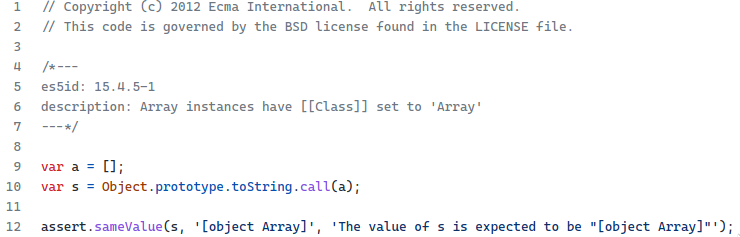
\includegraphics[width=1.0\textwidth]{images/test262_array_test.png}
    \caption{Test262 es5id: 15.4.5-1}
    \label{fig:Test262_example}
\end{figure}



%% metadados ja incluidos
%% referir outra vez o exemplo
% - metadados oficialmente incluídos nos testes
%   - que metadados é que os testes contém actualmente
The \texttt{Frontmatter} has keywords to hold metadata of the test. These keywords are associated with specific elements of metadata concerning the test. Bellow is the list of possible keywords and their meaning:

\begin{itemize}
\item \texttt{description} - contains a short description about what will be tested;
%
\item \texttt{esid} - contains the hash identifier of the ECMAScript portion associated with the feature that will be tested (the identifier references the most recent version of ECMAScript when the test is created);
%
\item \texttt{info} - contains a deeper explanation of the test behavior, frequently includes a direct citation of the standard;
%
\item \texttt{negative} - indicates that the test throws an error; associated to the keyword will be the type of error the test is supposed to be thrown (e.g. \texttt{TypeError}, \texttt{ReferenceError}) as well as the phase in which the error is expected to be thrown (e.g. \texttt{parse} vs \texttt{resolution} vs \texttt{runtime});
%
\item \texttt{includes} - contains the list of \texttt{harness} files that should be included in the execution of the tests (\texttt{Test262} makes use of a large number of auxiliary function defined in a dedicated library referred to as the \texttt{Test262} \texttt{harness} described later in this section);
%
\item \texttt{author} - contains the identification of the author of the test;
%
\item \texttt{flags} - contains a list of booleans for each test property, the properties being: (1) \texttt{onlyStrict}, the test is only executed in strict mode; (2) noStrict, the test will only be executed in mode \emph{sloppy}; (3) \texttt{module}, the test must be integrated as a \texttt{JavaScript} module; (4) \texttt{raw}, executes the test without any modification, which implies running as \texttt{noStrict}; (5) \texttt{async}, the test is contains asynchronous functions; (6) \texttt{generated}, the test generates the files specified by the property; (7) \texttt{CanBlockIsFalse} and (8) \texttt{CanBlockIsTrue}, the test will run if the property \texttt{CanBlock} of the \colorbox{orange}{\texttt{Agent Record}} executing it is false and true respectively; (9) \texttt{non-deterministic}, indicates that the semantics used in the test are intentionally under-specified and therefore the test passing or failing should not be regarded as an indication of reliability or conformance;
% QUESTION clarificar se e' necessario citar o que e' 'Agent Record' uma vez que nao vou explicar
%
%
\item \texttt{features} - contains a list of features that are used in the test;
%
\item \texttt{es5id} and \texttt{es6id} - indicates that the feature being tested belongs to ECMAScript 5 and 6 respectively and contains the hash identifier of the section of the standard it belongs to; these keywords have been deprecated and substituted by esid.
\end{itemize}


% Varias observacoes: 
%  - A metada esta muitas vezes INCOMPLETA e algumas vezes incorrecta 
%  - é preciso calcular a metadata certa
As Figure 5 illustrates, it is often the case that the metadata of a test is incomplete. Some tests also have the wrong metadata. As part of this thesis, we plan to process all the tests to check and correct their corresponding metadata as well as completing the metadata that is \colorbox{orange}{missing.}

%% QUESTION juntar os paragrafos?

%% metadados que achamos relevantes e nao estao incluidos
%% ...
\colorbox{orange}{The example} in Figure \ref{fig:Test262_example} has 2 keywords, description and the deprecated es5id. Besides the obvious upgrade from \texttt{es5id} to \texttt{esid} it would be useful to have \texttt{includes} with the \texttt{harness} files needed to execute the test. The \texttt{harness} information is very useful since it makes it easy to identify the part of the \texttt{harness} needed to run that test, opening the door for loading only part of the \texttt{harness} instead of the whole \texttt{harness} which is the current approach.



% - quais são os metadados que nós achamos serem relevantes e que estão em falta
\paragraph{New Metadata}
Besides the metadata that Test262 tests currently include, it would be useful for them to have additional information regarding:

\begin{itemize}
    \item \texttt{syntactic construct} - list of all syntactic constructions used in the test;
    \item \texttt{version} - the ECMAScript version of the standard in which the feature being tested was introduced;
    \item \texttt{built-ins} - list of all the built-ins used in the test.
    \item \texttt{harness-functions} - list of all the harness functions required to run the test.
\end{itemize}

This above metadata critical for filtering the tests when considering partial implementations of the language. For instance, if a JS engine only supports the 5th edition of the standard, one must be able to obtain all the corresponding tests for that \texttt{version}. Analogously, if a JS engine only implements certain \texttt{built-in} objects, one has to be able to filter out the tests that make use of the \texttt{built-in} objects that it does not implement. This would provide consistency and standardization to the selection of applicable tests to a partial implementation of the standard.
%
As for the \texttt{harness-functions}, it provides important information about the functions of \texttt{harness} that are used in the test. That information is relevant because only a small part of the \texttt{harness} is need in each test even though the whole library is loaded and tested. The harness has a total of 7290 lines in 32 files and is tested by 96 tests. By only including the exact functions that a test requires, one can speedup the testing process significantly.
% harness - has 32 files total 7290 lines (comments and blanck lines included)
% harness tests - has 96 files total 2646 lines (comments and blanck lines included)



\subsection{MetaData262 v0}
\label{subsec:MetaData262 v0}



% Para1 --> introduzir o trabalho do Miguel Trigo 
This thesis continues the master thesis of Miguel Trigo\cite{Thesis_Miguel_Trigo}, in which he developed a preliminary version of \texttt{MetaData262}. More specifically, he built a MongoDB database storing the metadata of all Test262 tests, representing the metadata of each test as a JSON object.



% Para2 --> estrutura da metadata
In \texttt{MetaData262 v0}, each test is associated with a JSON object storing the various metadata properties of the test and their corresponding values, with those metadata properties being the keywords of the \texttt{Frontmatter} mentioned in the previous section.
%
Besides the existing metadata properties, various new properties were added to \texttt{MetaData262 v0}. We can divide these new properties into 3 main groups: location properties, extra front matter properties, and statistics properties. Each of these groups will be discussed next.

% Para 2.1 [path] (location)
\paragraph{Location group}
The location group contains information about the path to the test inside the \texttt{Test262}. It consists of the properties \texttt{path}, storing the relative path to the test starting at the root of the \texttt{Test262} project, and splitPath, storing the array obtained by splitting the \texttt{path} string into its corresponding folders.


% Para 2.2 [extra front matter: syntactic constructs, built-ins, version] 
\paragraph{Extra front matter group}
The extra front matter group contains new metadata generated for \texttt{MetaData262 v0}. The new metadata generated is associated with the properties: \texttt{syntactic\_constructs}, \texttt{version}, and \texttt{builtIns} that were mentioned in the previous section as important metadata to add. The property \texttt{version} stores the \texttt{ECMAScript} standard version the test belongs to. The property \texttt{syntactic\_construct} stores an array with all the syntactic constructions that the test contains. As for \texttt{builtIns}, it stores all the built-ins that the test interacts with, mapping each built-in to its fields and methods used by test. 


% Para 2.3 [statistics]
\paragraph{Statistics group}
Finally, the statistics group contains some statistical data about the tests. It contains the properties: \texttt{asserts}, \texttt{error}, \texttt{esprima}, and \texttt{lines}. The \texttt{asserts} property holds the amount of \texttt{assert} statements in the test. The \texttt{error} property stores the amount of calls made to \texttt{Test262} error functions. The \texttt{esprima} property stores a boolean value indicating whether or not the Esprima\cite{Esprima} parser supports the test. \texttt{Esprima} is a standard-compliant \texttt{ECMAScript} parser fully developed in \texttt{ECMAScript}; \texttt{Esprima} fully supports up to version 7 of the standard. The property \texttt{lines} holds the number of lines of code the test has, excluding comments and empty lines.



\subsubsection{Example}

% Para3 --> exemplo da MetaData262 v0
Figure \ref{fig:json_metadata} shows the JSON object storing the metadata generated from the Test262 test given in Figure \ref{fig:Test262_example}. 
% Observacoes sobre o exemplo 
The JSON object begins with the \texttt{path} property storing the path to the test at hand. After, the \texttt{version} property indicates that this test belongs to the fifth version of the standard. If \texttt{MetaData262 v0} was not able to compute the version of the test, this field is omitted. Next, we have the properties corresponding to the test's \texttt{Frontmatter} (note that the deprecated \texttt{es5id} is replaced to the \texttt{esid} property).
% ignorar as propriedades buit-ins e Array
Next we have the \texttt{static\_constructs} property that holds an array with the syntactic constructors of the test. The \texttt{builtIns} property holds a JSON object, in which, each property corresponds to a built-in mapped to its functions and fields that are interacted with in the test. Finally, we have the statistics group of properties. The \texttt{asserts} property indicates that this test uses one assert statement. The \texttt{error} holds the numeric value zero since this test uses no error functions of \texttt{Test262}. The \texttt{esprima} property indicates this test is supported by \texttt{Esprima}. Finally, the \texttt{lines} property indicates that this test has 3 lines of code. Note that the example in Figure \ref{fig:Test262_example} splits the last line of the test in order to improve the readability of the figure hence only 3 lines are counted in the actual test).


\begin{figure}[ht]
    \centering
    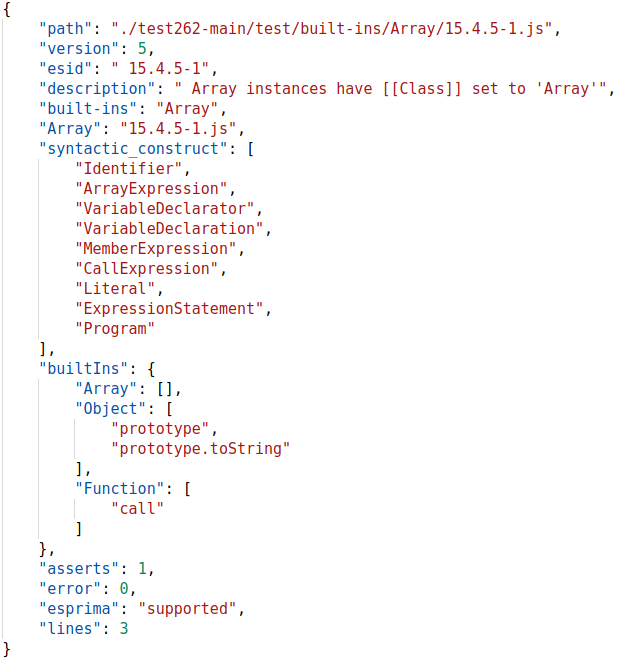
\includegraphics[width=0.9\textwidth]{images/json_metadata.png}
    \caption{Metadata generated for test esid: 15.4.5-1.js}
    \label{fig:json_metadata}
\end{figure}



\subsubsection{Metadata Computation}

% Para4 --> a metada original em falta teve de ser calculada e os 
% // bem como os novos campos da metadata -> 
As part of the setting up of MetaData262 v0,  M. Trigo had to compute the missing \texttt{Frontmatter} properties as well as the values of the new properties that he introduced. In most cases, the computation was straightforward, only involving a simple syntactic analysis of each test. However, the computation of the version and the built-ins used in each test was more involved. We will go through this process in more detail below.

% Para5 --> Version Computation 
\paragraph{Calculation of Version metadata}
The \texttt{version} of the standard a test belongs to is calculated using 3 different approaches: dynamic, static, and hybrid.Below we give a brief overview of each method:

\begin{itemize}
  \item \emph{Dynamic Approach:}
The dynamic approach is based on the waterfall model, running the tests in various JS engines, each corresponding to a specific version of the standard. As Figure \ref{fig:waterfall_model} illustrates, \texttt{MetaData262 v0} starts by running each test in the JS engine corresponding to version 5 of the \texttt{ECMAScript} standard (represented as ES). If the test output is correct then the test is labelled as belonging to version 5 of the standard, otherwise the test will be run in the engine implementing the next version of the standard. This process repeats until the last engine, associated with version 11 of the standard. If the test output is not the expected again, then the test is not supported.
%
  \item \emph{Static Approach:}
The static approach determines the version of a test by analyzing the static keywords of the test. Essentially, a test is labeled with the version corresponding to the keyword with the latest associated version; formally:
\[version(test) = max \{ version(keyword) | keyword \in test \} \]
For instance, if a test contains two keywords introduced in versions 6 and 8, then the test will belong to the version 8 of the standard. \texttt{MetaData262 v0} implements the static approach in the following way. It maintains an internal map associating each keyword with the version in which it was introduced. Given a test to be labeled, \texttt{MetaData262 v0} first computes the AST of the test using the \texttt{Esprima} parser and then traverses the AST to obtain all the keywords used in the test. Finally, it labels the test with the version of the latest keyword (as discussed above). 
%
  \item \emph{Hybrid Approach:}
The hybrid approach is calculated using the results of the dynamic and static approaches. The hybrid approach merges the results by maintaining the higher version detected between each approach for each test. For instance, if the dynamic approach's result for a test is version 6 and the static's result for the same test is version 8, then, the test is labeled as belonging to version 8 of the standard according to the hybrid approach.
\end{itemize}


\begin{figure}[ht]
    \centering
    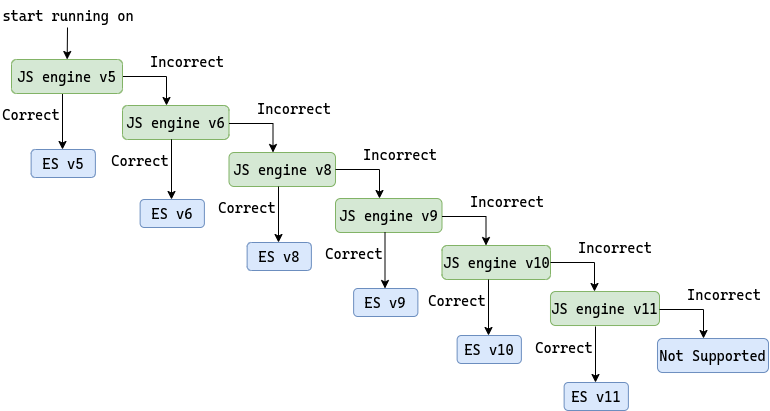
\includegraphics[width=1\textwidth]{images/waterfall_model.png}
    \caption{Waterfall model of the dynamic approach to calculate the ECMAScript version}
    \label{fig:waterfall_model}
\end{figure}



% Para6 --> Built-in Computation 
\paragraph{Calculation of built-ins metadata}
The \texttt{built-ins} used by each test are calculated using two separate approaches: dynamic and static. As in the calculation of the \texttt{ECMAScript} version both approaches are combined to improve the results. Below, we describe each approach separately:

\begin{itemize}
  \item \emph{Static Approach:}
The static approach maintains an internal map associating each built-in method and property with the name of the corresponding  built-in object (e.g. the method hasOwnProperty is associated with the built-in object \texttt{Object}). The static approach first computes the AST of the test using \texttt{Esprima} and then traverses the AST checking for each method and property for the built-in object it is associated with. In the end, it outputs a JSON object mapping each built-in object to an array with the names of its methods and properties that the test uses. 
%
  \item \emph{Dynamic Approach:}
The dynamic approach works by running the actual code of the test and logging the interactions of the test with the JavaScript built-ins. To this end, \texttt{MetaData262 v0} wraps the methods of every built-in object in an auxiliary function that calls the corresponding methods and adds an entry to the log registering that call. Finally, \texttt{MetaData262 v0} analyses the log information to determine the built-in methods used by the test. 
\end{itemize}



\section{Related Work}
\label{sec:Related Work}



\section{Design and Methodology}
\label{sec:Design and Methodology}



We recall that this thesis has two goals. Firstly, we want to improve \texttt{MetaData262 v0} in two ways: add support for missing metadata elements, and improve the infrastructure for the metadata computation, making the obtained metadata more reliable and the process faster and reproducible. Secondly, we want to create a visualisation system for easy selection of tests and display of test statistics.


\subsection{Improvements to MetaData262 v0}
\label{sub:improvements_to_metadata262_v0}


% Para1 --> problemas do calculo da metada existente na Metadata262 v0. 
% --> as versoes estao mal calculadas porque nao existem JS engines 
% que implementem exactamente uma versao e so essa versao 
% --> versoes calculadas em instalacoes ad-hoc 
% -- é preciso melhorar a analise dinamica considerando mais JS engines 
% --> os built-ins tb estao mal calculados porque a analise dinamica 
% dos built-ins ignora propriedades -> so considera chamadas a funcoes 
% por isso, se um teste for apenas: Array.prototype.pop = 3; 
% nao vai ser identificado como um teste que usa o array pela analise 
% dinamica 
% --> ha informacao em falta 
% ficheiros da harness e funcoes da harness
% data de criação do teste 
The metadata calculated by \texttt{MetaData262 v0} is flawed in several ways: in the version calculation, in the built-in calculation, and in the harness calculation. We describe these flaws and how to fix them in more detail next.

\begin{itemize}
\item \emph{Version Calculation} - The version calculation is flawed in both the static and dynamic approachs, meaning that the hybrid approach that uses the results of the previous two will also be compromised. The static approach is flawed since the \texttt{Esprima} parser only fully supports up to \texttt{ECMAScript} version 7. Improvements can be made by finding a \texttt{JavaScript} parser that supports a later version of the standard. The dynamic approach's flaw lies in the way it works, since there is no JS engine that fully supports a version of the standard and only that one. To improve the dynamic approach we will add more JS engines. By adding more data points to the calculation, we will increase the reliability of the obtained metadata.
%
\item \emph{Built-in Calculation} - The built-in calculation is also flawed in both the static and dynamic approachs. The static approach has the same flaw since it also uses \texttt{Esprima} as parser. Therefore the same improvement can be made by finding a newer parser. As for the dynamic approach, it is flawed due to the fact that only function calls are logged and therefore detected. If the properties of a built-in are changed directly then it will not be detected. For example if a test preforms \texttt{Array.prototype.pop = 3;} then the property \texttt{prototype} of the Array built-in will be changed even though no function call was made. This can not be detected by the current dynamic approach.
%
\item \emph{Harness Calculation} - The \texttt{harness} calculation is not done, including only the little information available in the \texttt{Frontmatter} of a few tests. This calculation can be improved by completing \texttt{includes} metadata and adding an additional \texttt{harness-functions} metadata. Both \texttt{includes} and \texttt{harness-functions} are mentioned in earlier sections, the first stores the files of the \texttt{harness} needed to run the test and the second will store the functions from those files that are actually used in the test.
\end{itemize}


% Para 2 --> Scalability/Performance and Replicability of the calculation
% 5.1 - Precise Metadata for test262 tests 
% --> calcular a metadata precisamente e de forma facilmente reproducible 
% 5.1.1 versao -> 
% Montar um sistema escalavel para o calculo das versoes 
% associamos a cada versao um numero arbitrario de docker images cada uma 
% com um JS engine supostamente dessa versao 
% ---> parelelizacao etc
% 5.1.2 built-ins -> melhorar a instrumentcao para o calculo dinamico dos 
% built-ins --> em particular, apanhar property look-ups dinamicamente
The improvements the \texttt{MetaData} calculation precision, in particular the version dynamic approach, will enhance the issue of performance. This issue will be improved with the use of \texttt{docker}\cite{docker} containers and this way we will also improve the ease to replicate the calculations of the \texttt{MetaData}.
%
The duration to calculate the version with the dynamic approach scales linearly with the amount of engines per standard version being used. In \texttt{MetaData262 v0} only two JS engines are being used and the dynamic approach already takes multiple hours to run.
%
With the use of \texttt{docker} containers we will be able to parallelize the work of the dynamic approaches by multiplying the docker images that run the JS engines. Containers running in parallel will not only improve the performance but also allow MetaData262 to be replicated in an easier way since it requires a smaller configuration effort to replicate the \texttt{MetaData} calculation.
% TODO rescrever comentarios do prof


\subsection{MetaData262 Visualization System}
\label{sub:metadata262_visualization_system}

% --> Problemas de acesso a metadata e obtencao de informacao estatistica 
% sobre os testes 
% --> neste momento quem quiser obter informacao estatisca sobre os 
% testes tem de interagir com uma base de dados Mongo e depois processar a informacao 
% como entender
% O objectivo desta tese é resolver estes dois problemas.

% Para 0 --> Motivar a criacao do system de visualizacao
The \texttt{MetaData262 Visualization System} appears to ease the barrier to access the \texttt{MetaData262 v0} information and statistics. Right now the metadata is hosted in a MongoDB database leading to the need to have knowledge of MongoDB to get the information. After getting the information there would most likely be a need to process that metadata and maybe even generating charts to provide statistics. This is visualization system will make this process much easier.

% 5.2 - MetaData Visualisation System 
% portal para visualizacao da metadata dos testes + informacao estatisca sobre os testes 
% --> gerar automaticamente 
% --> print screens do que ja fez
% --> discussao das bibliotecas que vai considera usar para criacao e display 
% da informacao estatisca
% --> Exemplos de graficos a gerar 
% -- ...

% Para 1 --> O que o website vai mostrar e o que para isso e' necessario fazer
The \texttt{MetaData262 Visualization System} is in its core a web application that allows users visualize and filter the \texttt{Test262} metadata easily. The system will also update itself whenever there are changes in \texttt{Test262}. Users are able to filter the metadata by the built-ins and version of the test. Users will also be able visualize the queried information in different ways: \texttt{PATH}, \texttt{JSON}, and \texttt{STATS}. The \texttt{PATH} will only show the path to the tests in \texttt{Test262}. The \texttt{JSON} will allow the users to see the full metadata calculated for the tests. Finally, the \texttt{STATS} will show some statistics about the tests queried. To ensure that the information is up to date, this system needs to update itself since this is a thesis project and there is no active developer team. In order to accomplish that, the system will need check for changes, be it in the form of new tests or changes to existing ones, and calculate the new metadata.


% Para 2 --> O que ja esta feito
The development of the web application has already began, \colorbox{orange}{Figure} \ref{fig:website} shows the progress already made. The image has 2 main parts: the filters part, and the information part.
%
The upper part is the filters part, where it is possible to select the filters for querying the metadata. The first filter, \texttt{BuiltIn Belongs} allows to select tests from the subfolders of the built-in folder in the \texttt{Test262}. The \texttt{BuiltIn Contained} enables the user to filter tests by the built-ins the tests can use.
%
The \texttt{BuiltIn Belongs} and \texttt{BuiltIn Contained} filters are combined using \texttt{AND} or \texttt{OR} relations. The \texttt{AND} relation will only return tests that satisfy both filters. As for the \texttt{OR} relation, it will return every test that satisfies either of the filters.
%
Then, we have the \texttt{Version} filter that allows filtering the tests by the \texttt{ECMAScript} version. Next, we have the \texttt{BACKEND SEARCH} and \texttt{LOCAL SEARCH} search buttons that will query the metadata database for the tests that satisfy the filters set. The \texttt{BACKEND SEARCH} filter the tests in the backend server while the \texttt{LOCAL SEARCH} it will filter the tests in the machine that is used to access the website.
%
In the example, the filters selected are \texttt{Object}  and \texttt{Array} for the \texttt{BuiltIn Belong} and \texttt{BuiltIn Contained} respectively with an \texttt{AND} relation and the sixth version is also selected.
%
The information part of the image contains the result of the query. The information can already be displayed in two of the three ways mentioned above, in the image the \texttt{PATH} is selected. The image also shows it took 16 milliseconds to have the query results available to the user. The image displays that a total of 32 tests satisfy the filters selected. The image shows the path of the tests selected. Note that not all tests are shown at the same time, in order to improve performance only 10 tests are shown at a time, at the bottom of the image is the pagination menu.
% QUESTION mudar o titulo do website para MetaData262 Visualization System ??


% printscreens do site 
\begin{figure}[ht]
    \centering
    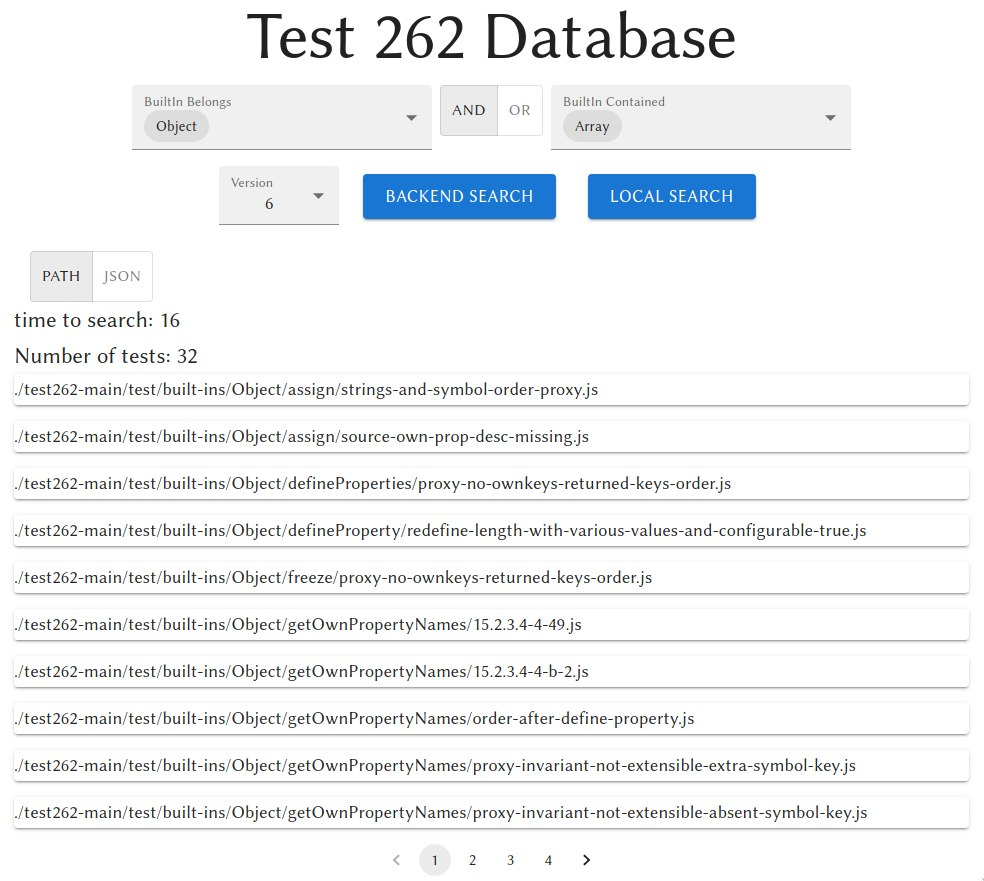
\includegraphics[width=1\textwidth]{images/website.png}
    \caption{Website for searching the metadata in construction}
    \label{fig:website}
\end{figure}


% TODO rescrever tudo com comentarios do prof
% Para 3 --> Trade off the fazer a filtragem local or no servidor
In Figure \ref{fig:website} there are two search buttons because there at the time trade offs being made with either way of searching, the following results were run in the laptop serving the web application. The backend search starts getting slow whenever the amount of tests being returned surpasses 2500 in the local machine, taking on roughly half a second to get the results. The local search has the problem that it takes around 4 seconds to get all the metadata from the server at page load. The local search has the advantage of filtering the tests in a few milliseconds. Caching the metadata in the users browser would allow the metadata to be only loaded one, making the usability of the web application much better.

% TODO rescrever tudo com comentarios do prof
% Para 4 --> Os graficos que queremos gerar --> bibliotecas
This web application will allow the user to view charts about the metadata of the tests queried. M. Trigo's thesis he generated the charts shown in Figure \ref{fig:grafico_bigodes} and Figure \ref{fig:grafico_stackBar} as well as some other pie charts and bar charts. In the web application those charts will be generated in real time with the help of external libraries. Especially the charts below, the box and whiskers chart and the stacked bar chart, are not supported by many of the most popular libraries. Two of the libraries that are capable of generating all the charts needed are the \texttt{KendoReact}\cite{KendoReact} an UI library and \texttt{Victory}\cite{Victory} a chart library. \texttt{KendoReact} is a full UI library, charts being only part of its 126 components. Whereas, the \texttt{Victory} library has only 34 components and all are directly related with generating charts. The Victory library also seams simpler to use, the community around it seams more active which would be important in case of difficulty while implementing the charts needed.


\begin{figure}
\centering
\begin{minipage}{.5\textwidth}
  \centering
  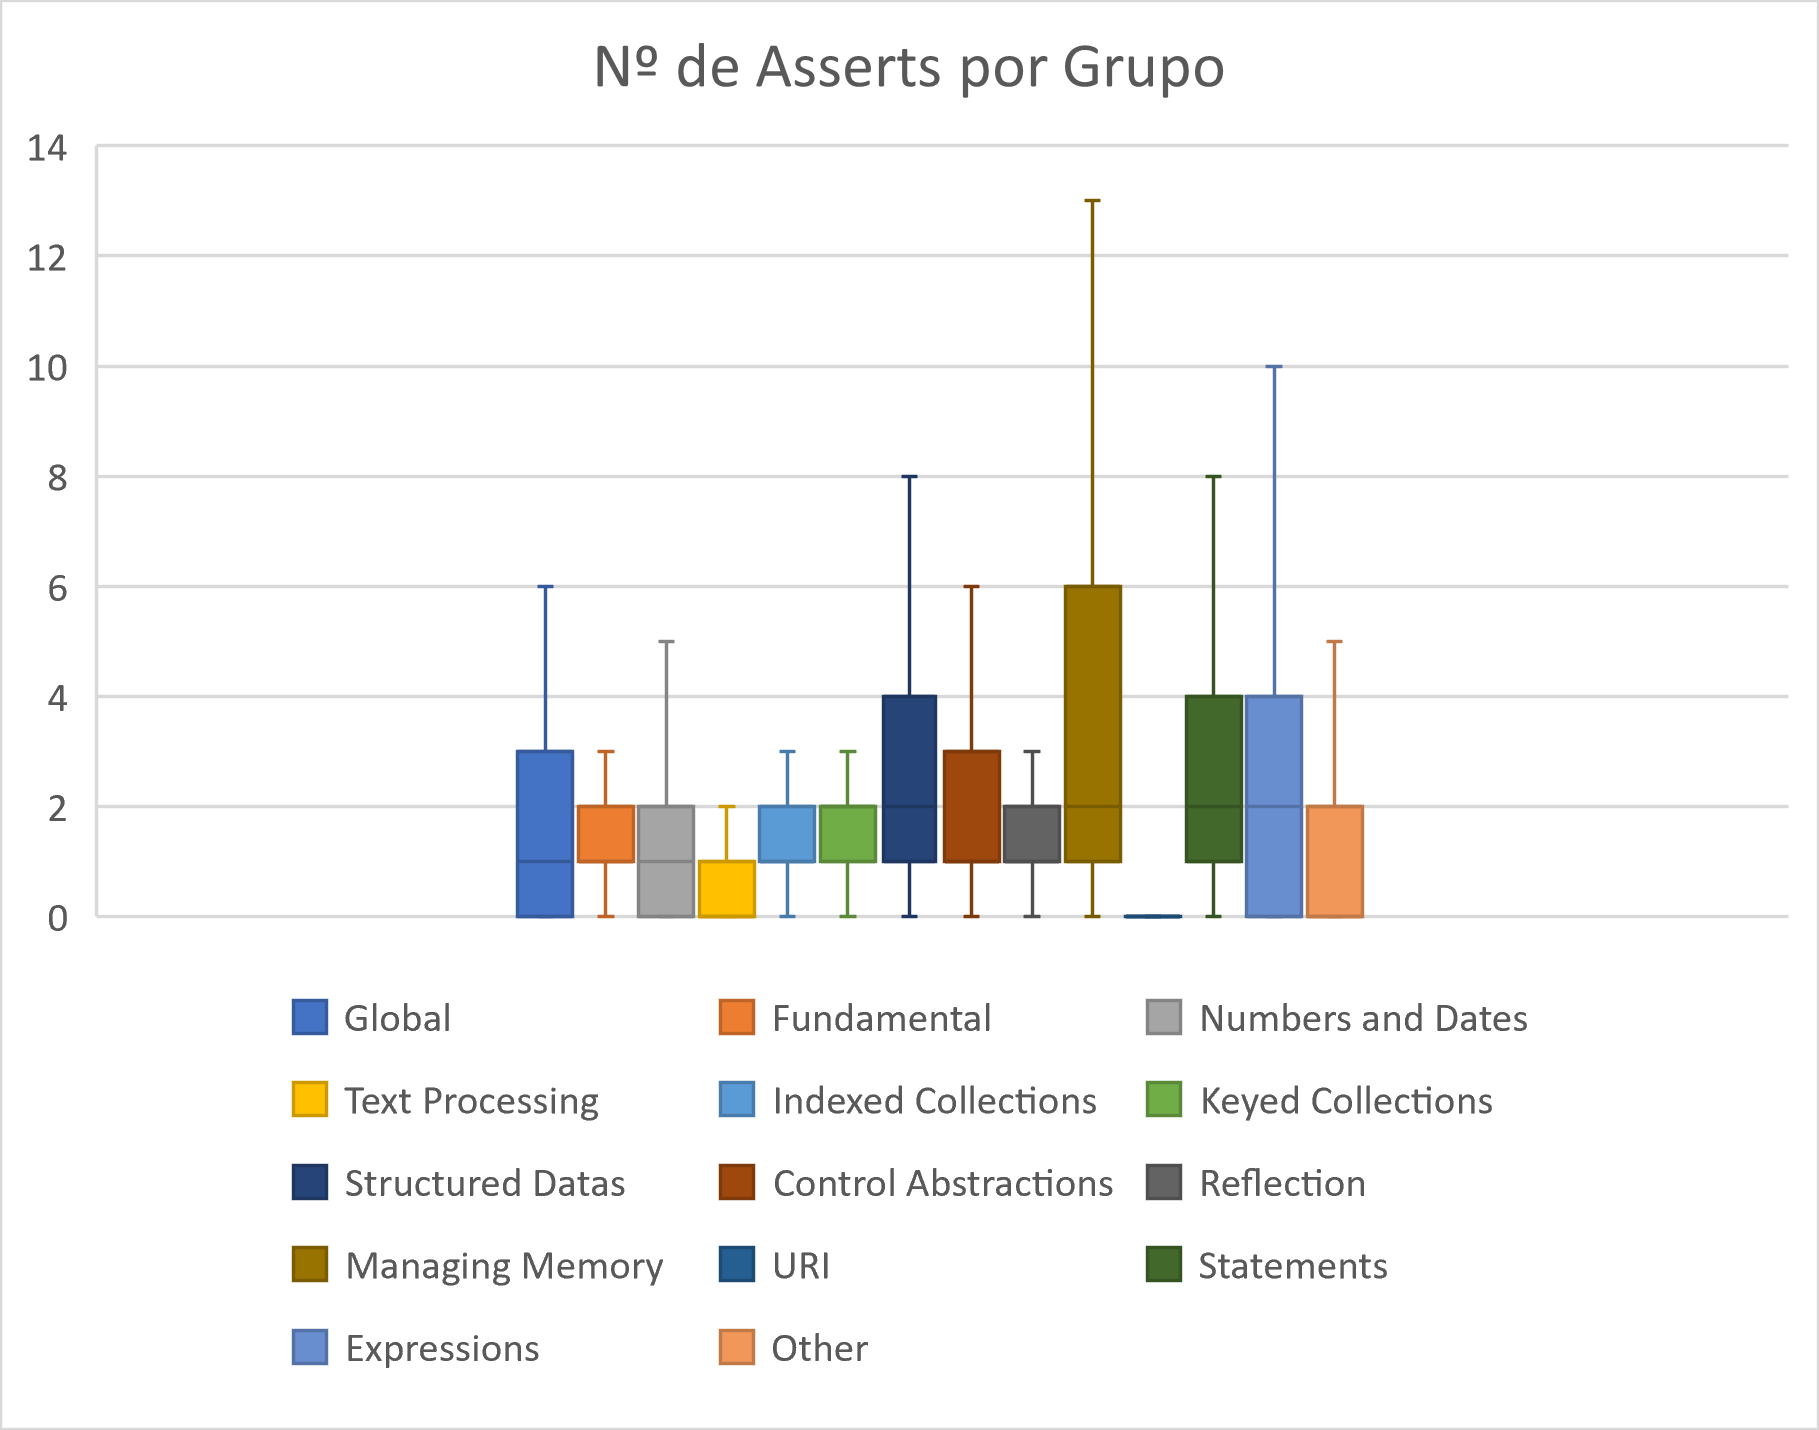
\includegraphics[width=0.95\textwidth]{images/n_asserts.png}
  \captionof{figure}{M. Trigo chart number of asserts by category}
  \label{fig:grafico_bigodes}
\end{minipage}%
\begin{minipage}{.5\textwidth}
  \centering
  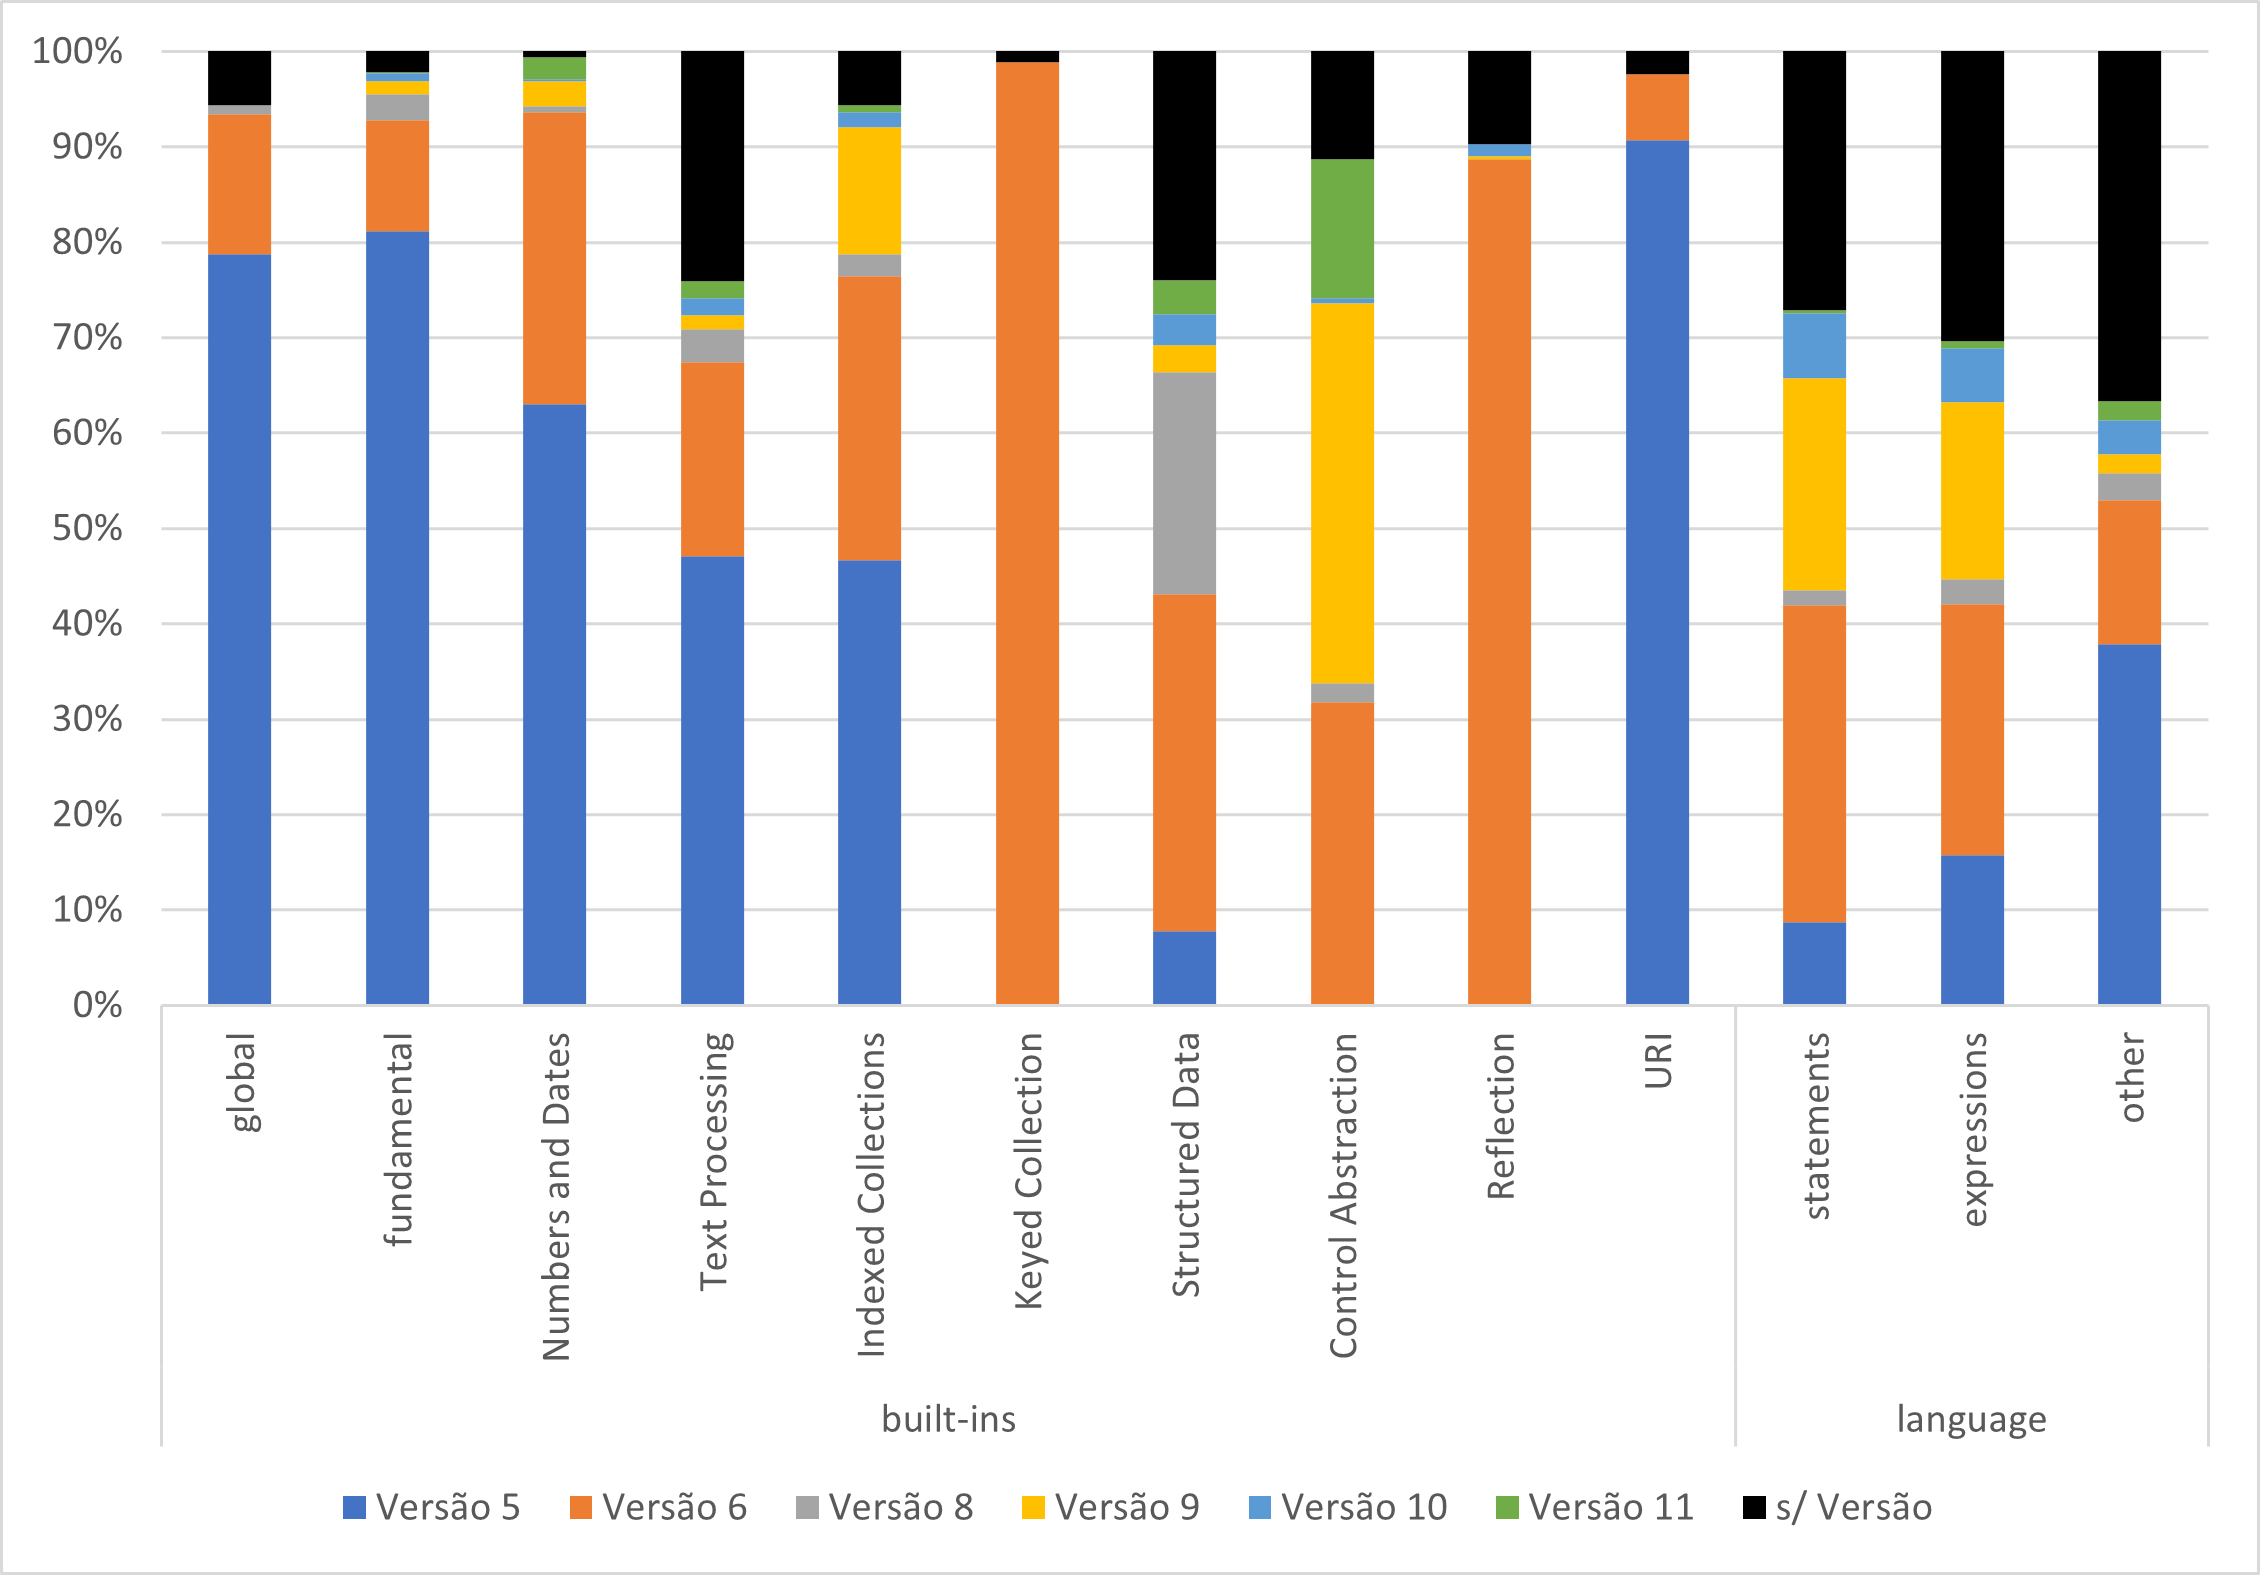
\includegraphics[width=0.95\textwidth]{images/version.png}
  \captionof{figure}{M. Trigo chart versions by category}
  \label{fig:grafico_stackBar}
\end{minipage}
\end{figure}


% Para 5 --> breve descricao do processo para manter a metadata atualizada
% ignorado por estar com 3 paginas so' sobre o website


\section{Evaluation and Planning}
\label{sec:Evaluation and Planning}


% Evaluation 
% - Discutimos avaliação das duas componentes do projecto 

% Componente 1 -> sistema para calculo da metadata
% É muito difícil de avaliar porque não há ground truth -> nós não sabemos qual é a versão dos testes
% - vamos seleccionar um conjunto aleatório de testes e analisa-los à mão comparando a versão calculada com a versão que sabemos ser a versão do teste 
% - vamos tb determinar a versão utilizando à data em que o teste foi inserido na Test262 -> pela data sabemos a versão corrente -> vamos olhar particularmente para os testes em que a versão calculada difere da versão da data dos testes 
% -> Atenção que a versão à data do teste não é necessariamente a versão do teste -> mas dá uma indicação
% --> testes analisados manualmente são os testes para os quais há grandes discrepâncias entre a versão à data do teste e a versão calculada para o teste

% Componente 2 -> sistema de visualisacao
% -- testes unitários para testar as funcionalidades base da aplicação 
% -- end-to-end tests -> testes do front-end

% Para 1 --> components a serem testadas
This thesis we will make improvements to the metadata calculation of \texttt{MetaData262 v0} and create a visualization system for it. The metadata improvements are divided into precision and performance. The evaluation of this thesis contributions is described in more detail bellow.

% Para 2 --> Metadata calculation precision  
\paragraph{Evaluation of metadata calculation precision}
The precision of the metadata calculated is very hard to access since the is no ground truth available. For example the versions of the tests are not available. Thus, to evaluate the the metadata calculation we will select a small random group of tests to analyze manually and compare the the version calculated. A second evaluation will be made to the tests that have the biggest difference between the version calculated and the version that was the latest at the time the test was added to \texttt{Test262}. Firstly, we will find the date the test was added to \texttt{Test262} and associate it with the latest \texttt{ECMAScript} version at that time. After, we will select the tests with the biggest discrepancy between the versions. Finally we will preform a manual evaluation to ensure that the right version was calculated. Note that the version discrepancy is merely indicative as more the once tests were detected as missing and subsequently added to complement \texttt{Test262}.


% Para 3 --> Metadata calculation performance
\paragraph{Evaluation of metadata calculation performance}
To evaluate performance improvements made to \texttt{MetaData262 v0} we will compare the time needed to preform the metadata calculation. This must be ran in the same system and with the least concurrent processes running in order to make sure we have better results.

% Para 4 --> visualization system
\paragraph{Evaluation of the visualization system}
The visualization system evaluation will have three types of tests: unit tests, end-to-end tests and load tests. The unit tests will ensure the correctness and reliability of the system. The end-to-end tests will guarantee that the website interface works correctly. Finally, the load tests will allow us to estimate the amount of users that the systems can support.


\subsection{Planning}
\label{sub:planning}

% subsection planning (end)
% Planning -> usar texto equivalente ao Miguel Trigo 
% - Melhoria do sistema de calculo da metadata - 2 meses
% - Conclusão do sistema de visualização - 2 meses
% - Avaliação - 1 mês 
% - Thesis Writing - 2 meses 
% Julho - (Agosto férias) - Novembro

The Plan for this thesis is based on the tasks that need to be preformed in order to accomplish the objectives defined in section \ref{sec:Goals}. Thus, this thesis has 4 main task to accomplish: improving the metadata calculation, concluding the visualization system, Evaluating the results, and writing the thesis. The planning for these tasks is represented in the Gantt diagram in Figure \ref{fig:gantt} and each task is described in more detail afterwards. Note that the month of August has a grey background due to it being a vacations.

% gantt tese
\begin{figure}[ht]
    \centering
    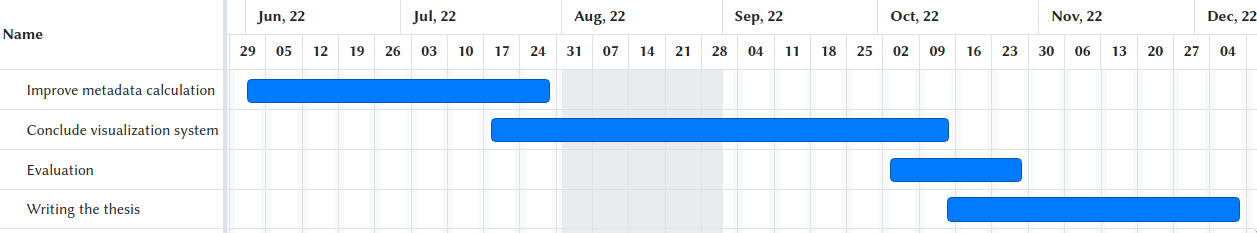
\includegraphics[width=1\textwidth]{images/gantt_thesis.png}
    \caption{Gantt diagram with the thesis plan}
    \label{fig:gantt}
\end{figure}

% gantt tese tempo dividido por mes
\begin{figure}[ht]
    \centering
    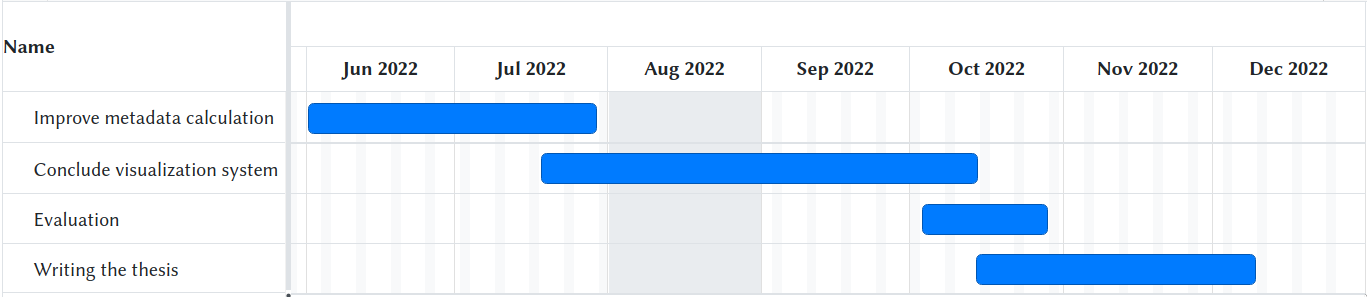
\includegraphics[width=1\textwidth]{images/gantt_thesis_month.png}
    \caption{Gantt diagram with the thesis plan}
    \label{fig:gantt_month}
\end{figure}


\paragraph{Improving metadata calculation}
This task consists of improving \texttt{MetaData262 v0} by improving its precision and performance as discussed in section \ref{sec:Design and Methodology}. The precision will be improved with more JS engines and a JS parser that supports more recent versions of the standard. As for the performance, we will parallelize the metadata calculation.

\paragraph{Concluding visualization system}
This task consists of concluding \texttt{MetaData262 v0} visualization system by adding the possibility to view statistics about the queried tests and improving the system's reliability through preparing it to handle wrong queries.

\paragraph{Evaluation}
This task consists of evaluating the results of the metadata generated. The most prone to error metadata will be checked by hand in order to guarantee the correctness of the results presented.

\paragraph{Writing the thesis}
This last task will consist in a report of the execution of the previous tasks. In the report we will present the results obtained as well as the conclusions reached after finishing this project. 


\section{Conclusion}
\label{sec:Conclusion}


%
% the environments 'definition', 'lemma', 'proposition', 'corollary',
% 'remark', and 'example' are defined in the LLNCS documentclass as well.
%

%
% ---- Bibliography ----
%
% BibTeX users should specify bibliography style 'splncs04'.
% References will then be sorted and formatted in the correct style.
%
% \bibliographystyle{splncs04}
% \bibliography{mybibliography}
%
\bibliographystyle{splncs04}
\bibliography{references}

\end{document}
